% Copyright 2017 by Jan Pluskal  <ipluskal AT fit.vutbr.cz>

\documentclass[10pt,xcolor=pdflatex]{beamer}
\usepackage{newcent}
\usepackage[utf8]{inputenc}
\usepackage{csquotes}
\usepackage{hyperref}
\usepackage{graphicx}
\usepackage{fancyvrb}
\usepackage{multirow}
\usepackage[backend=biber,maxbibnames=2,minbibnames=2, maxcitenames=2,mincitenames=2,sorting=ydnt,sortcites=true]{biblatex}
\addbibresource{./publications.bib}
\usetheme{FIT}


\newcounter{citeYearCounter}

\defbibcheck{intheyear}{
  \iffieldint{year}
    {\ifnumequal{\thefield{year}}{\theciteYearCounter}
      {}
      {\skipentry}}
    {\skipentry}}
\defbibenvironment{counting}
  {}
  {}
  {\xifinlist{\thefield{year}}{\yearlist}
    {}
    {\listxadd{\yearlist}{\thefield{year}}}}

%%%%%%%%%%%%%%%%%%%%%%%%%%%%%%%%%%%%%%%%%%%%%%%%%%%%%%%%%%%%%%%%%%
\title[Serious educational games by Olena Pastushenko, supervisor: prof. Ing. Tomáš Hruška, CSc]{Participatory development of serious educational games with dynamic difficulty adjustment}
\author[]{Olena Pastushenko \\Supervisor: prof. Ing. Tomáš Hruška, CSc. }
\institute[]{
Brno University of Technology, Faculty of Information Technology\\
Božetěchova 1/2. 612 66 Brno - Královo Pole\\
ipastushenko@fit.vutbr.cz}

\date{April 16, 2018}
% \date{\today}
%\date{} % no date

%%%%%%%%%%%%%%%%%%%%%%%%%%%%%%%%%%%%%%%%%%%%%%%%%%%%%%%%%%%%%%%%%%

\begin{document}

\frame[plain]{\titlepage}

%%%%%%%%%%%%%%%%%%%%%%%%%%% INITIALIZATION OF CITE ENUMERATION %%%%%%%%%%%%%%%%%%%%%%%%%%%%%%%%%%%%%%%
\begin{frame}<handout:0|beamer:0>
  \nocite{*}
  \gdef\yearlist{}%
  \begingroup%
    \makeatletter%
    \def\blx@driver#1{}%
    \printbibliography[env=counting,heading=none,sorting=ydnt]%
    \makeatother%
  \endgroup%
\end{frame}


\renewcommand*{\do}[1]{%
  \setcounter{citeYearCounter}{#1}%
  \begin{frame}[allowframebreaks]\frametitle{Publications #1}  
  \printbibliography[
  %title=#1
  %,heading=subbibliography
  ,check = intheyear]
  \end{frame}
  }
%%%%%%%%%%%%%%%%%%%%%%%%%%% REMARKS - HIDDEN SLIDES %%%%%%%%%%%%%%%%%%%%%%%%%%%%%%%%%%%%%%%

\begin{frame}<handout:0|beamer:0>
\frametitle{Pokyny od Radka Burgeta}
    Od doktorandů se očekává následující prezentace:
    \begin{itemize}
        \item  1. ročník: 5minutová prezentace na zamýšlené téma disertace.    
        \item  2. ročník: prezentace 8 minut, zaměřená na finalizaci PhD. Musí obsahovat hrubý obsah disertace, včetně kapitol spolu s procentuálním vyjádřením, co již je hotovo. Nesmí se krýt s obhajobou tezí, tzn. důraz na vlastní práci na disertaci, omezit současný stav problematiky apod.    
        \item  3. ročník a starší : prezentace 12 minut, popis finalizace PhD, musí obsahovat přesný obsah disertace, včetně kapitol spolu s procentuálním vyjádřením, co již je hotovo.
    \end{itemize}
   V prezentaci prosím explicitně vyznačte výsledky (publikace apod.) dosažené v tomto akademickém roce.
\end{frame}

\begin{frame}<handout:0|beamer:0>
\frametitle{Frame Title}
    Example \emph{content}.
\end{frame}


%%%%%%%%%%%%%%%%%%%%%%%%%%% Teaching Activities %%%%%%%%%%%%%%%%%%%%%%%%%%%%%%%%%%%%%%%

 \begin{frame}\frametitle{Teaching Activities}
     \begin{table}[]
     \centering    
     \label{my-label}     
     \begin{tabular}{|l|l|l|l|}
     \hline
     Year                       & Class                & Type    & CH \\ \hline
        \multirow{8}{*}{2017/18} & IIS                 & Project & 98,8  \\ \cline{2-4} 
                                & \multirow{3}{*}{ITW} & Lab     & 48  \\ \cline{3-4} 
                                &                      & Project & 56  \\ \cline{3-4}
                                &                      & Exam    & 10,5  \\ \cline{2-4}
                                & WAP                  & Project & 65  \\ \cline{2-4} 
                                & \multirow{2}{*}{}    & SP      & 12  \\ \cline{3-4} 
                                &                      & BP      & 36  \\ \cline{1-4} 
                                &                      & Summary & 326,3  \\ \hline
     \end{tabular}      
     \caption{Teaching activities overview.}
     \end{table}
 \end{frame}
 
 %%%%%%%%%%%%%%%%%%%%%%%%%%% Accomplishments %%%%%%%%%%%%%%%%%%%%%%%%%%%%%%%%%%%%%%%

 \begin{frame}\frametitle{Accomplishments}
     \begin{itemize}
         \item Article presentation at WorldCIST'18 conference
         \item Collaboration on writing the project task and computer exersices for ITW
         \item Development of new gamified computer exercise for learning jQuery for ITW students
         \item Created presentation about grid layouts and CSS frameworks usage for ITW course
         \item Questionnaires studies about students satisfaction with the new exercises approach
     \end{itemize}
 \end{frame}
 
 %%%%%%%%%%%%%%%%%%%%%%%%%%% Cooperation on Grants %%%%%%%%%%%%%%%%%%%%%%%%%%%%%%%%%%%%%%%
 
 %  \begin{frame}\frametitle{Cooperation on Grants}
 %     \begin{itemize}
 %         \item Employed on grant AAA
 %         \begin{itemize}
 %            \item 0.5 work load
 %            \item Coding software
 %            \item Invited speech at XXX conference
 %         \end{itemize}
 %         \item Employed on grant BBB
 %         \begin{itemize}
 %            \item 0.25 work load
 %            \item Writing papers
 %            \item 2x FIT-BUT internal presentations
 %         \end{itemize}         
 %     \end{itemize}
 % \end{frame}


%%%%%%%%%%%%%%%%%%%%%%%%%%% Publications %%%%%%%%%%%%%%%%%%%%%%%%%%%%%%%%%%%%%%%
\begin{frame}<handout:0|beamer:0>
  Vsechno napiste do publications.bib ...
  \begin{enumerate}
      \item SW vystupy
      \item Postery
      \item Prezentace!
  \end{enumerate}
  Vse se da zadat i do WISu jako typ prezentace s 0b, SW vystup do software, atd \dots
\end{frame}

\dolistloop{\yearlist}

%%%%%%%%%%%%%%%%%%%%%%%%%%% Publication Summary %%%%%%%%%%%%%%%%%%%%%%%%%%%%%%%%%%%%%%%

\begin{frame}\frametitle{Publication Summary}
\begin{table}[]
\centering
\label{my-label}
\begin{tabular}{|l|l|l|l|l|}
\hline
Type             & Accepted & Rejected & Review & Total \\ \hline
Conference paper &   1      &   0      &  0     &  1    \\ \hline
Journal entry    &   0      &   0      &  0     &  0    \\ \hline
Invited speech   &   0      &   0      &  0     &  0    \\ \hline
Software         &   2      &   0      &  0     &  2    \\ \hline
Poster           &   0      &   0      &  0     &  0    \\ \hline
...              &   0      &   0      &  0     &  0    \\ \hline
\end{tabular}
\caption{Summary of overall publication activities.}
\end{table}
\end{frame}

%%%%%%%%%%%%%%%%%%%%%%%%%%% Idea %%%%%%%%%%%%%%%%%%%%%%%%%%%%%%%%%%%%%%%

\begin{frame}\frametitle{Idea}

% Ideálně vše shrnující obrázek o tématu dizertace
   \begin{figure}[h!]
    \centering
      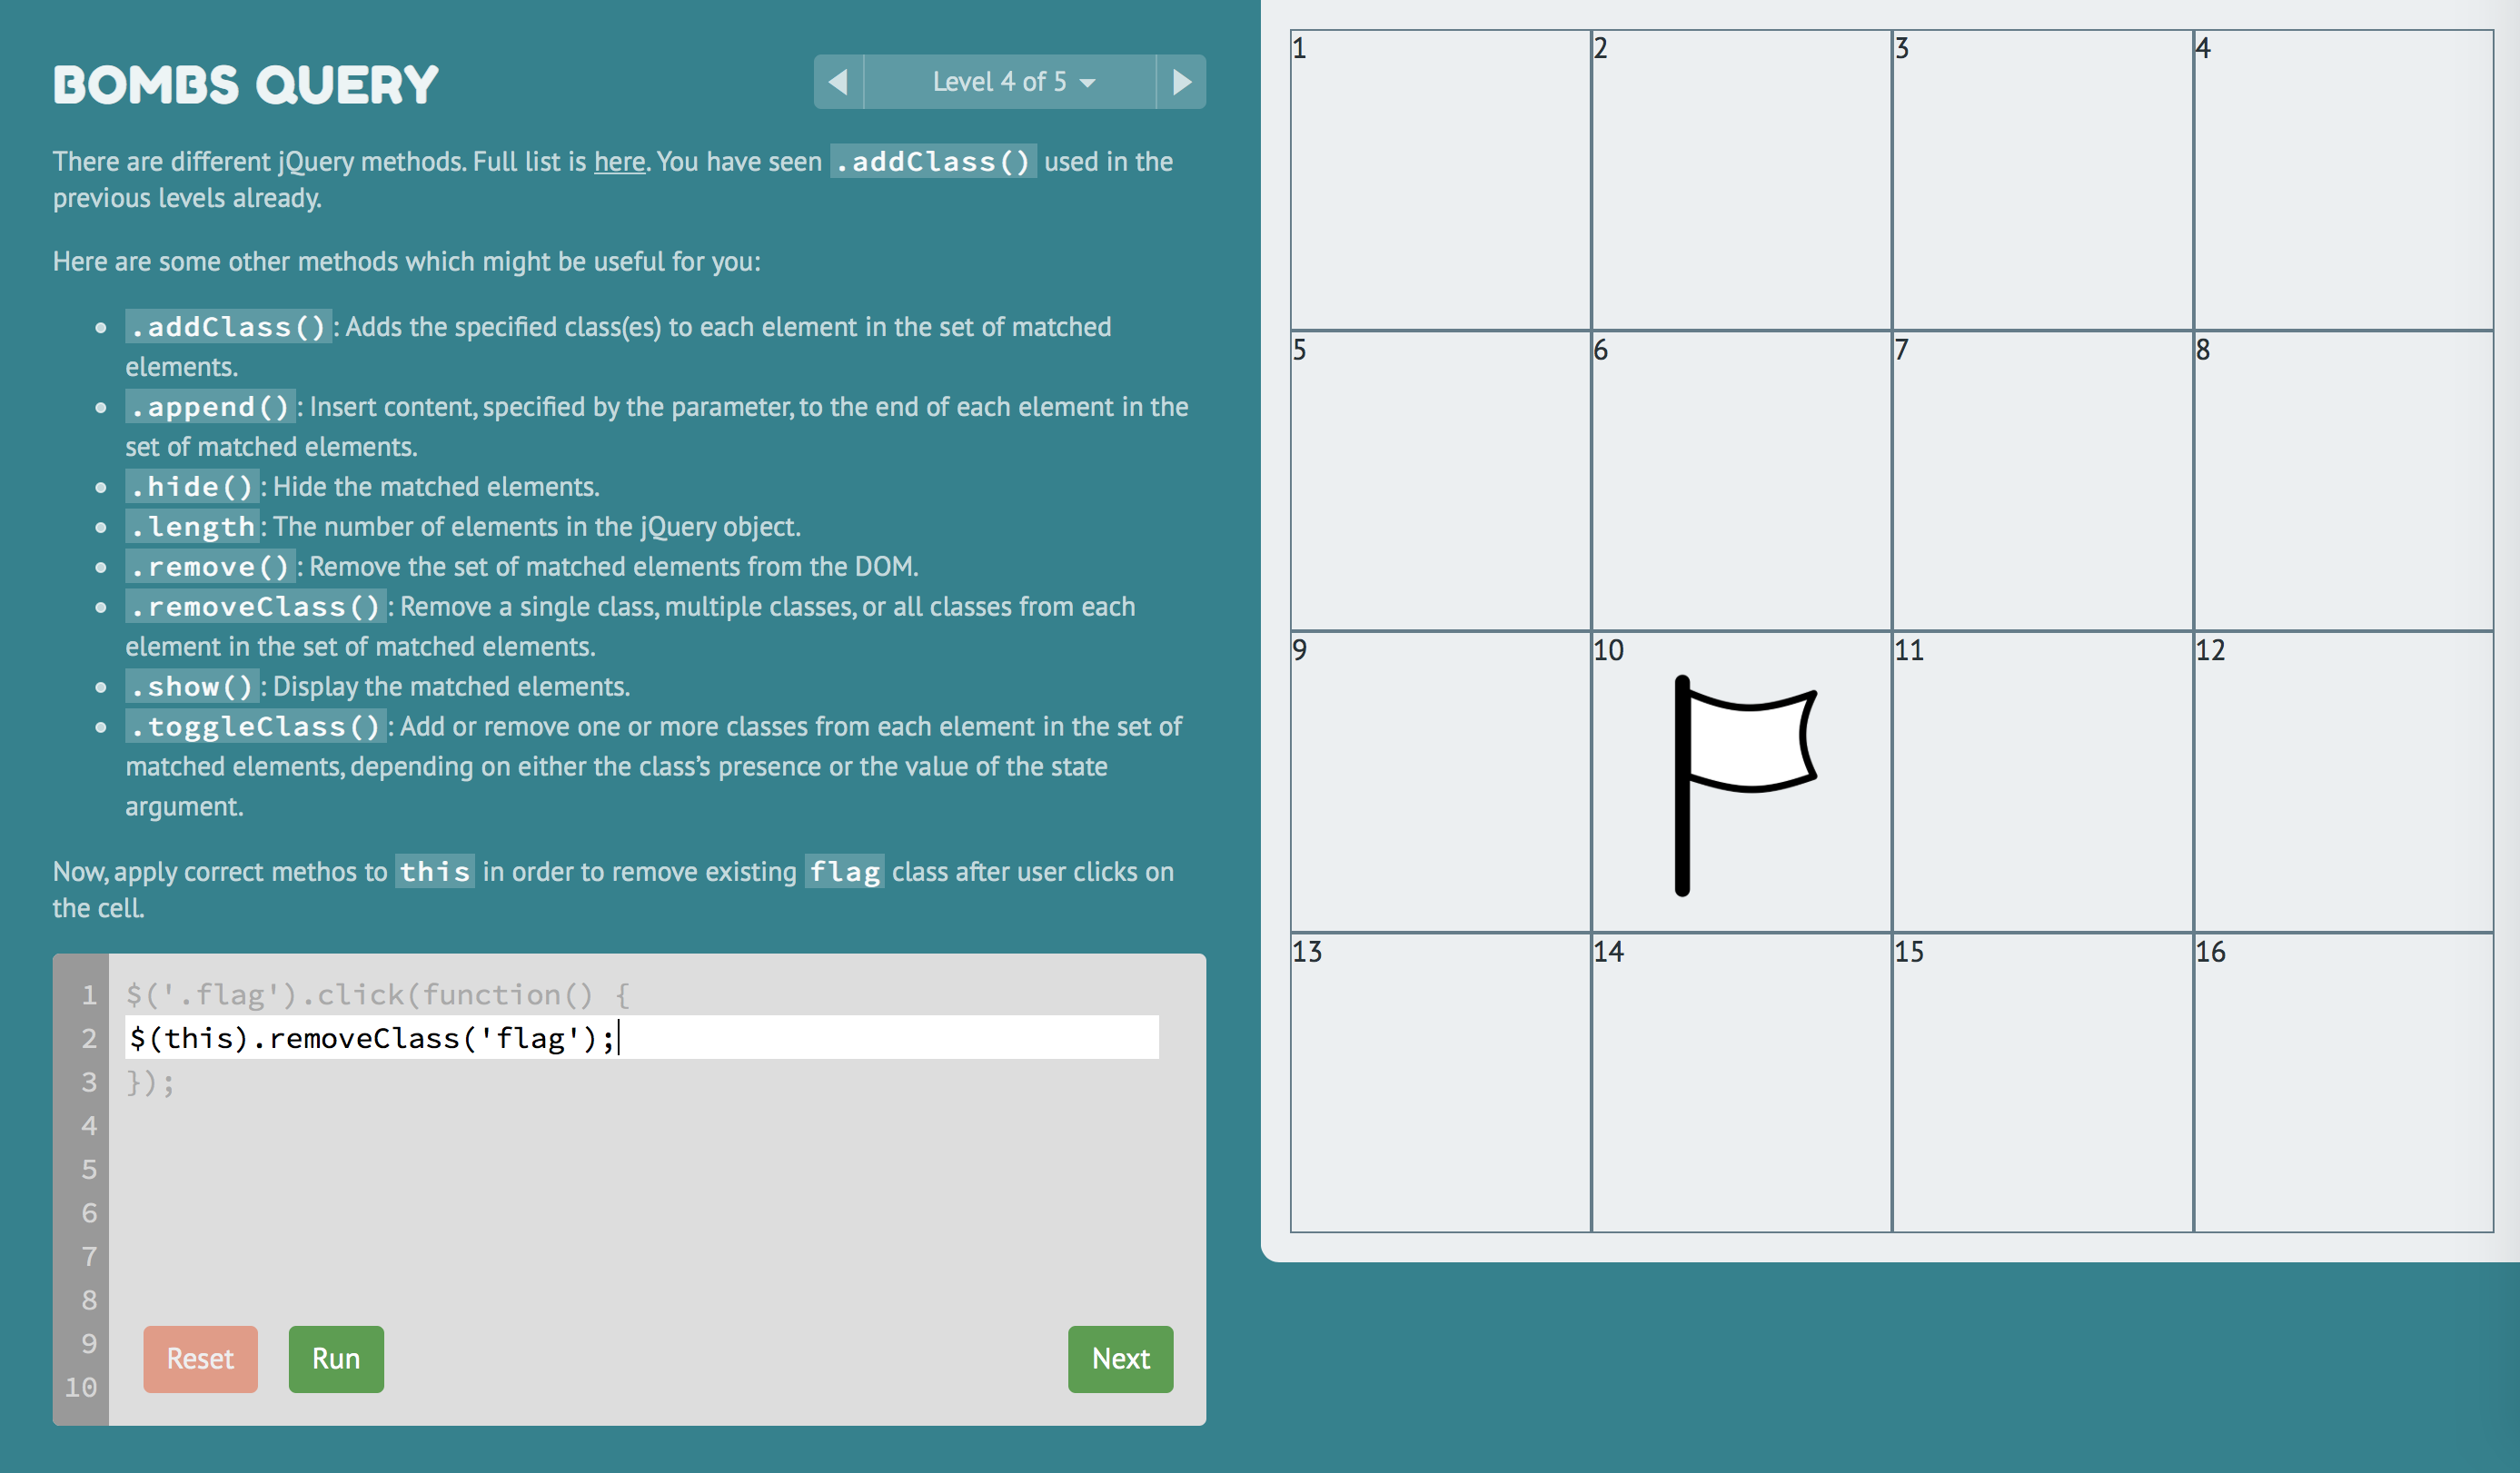
\includegraphics[width=0.9\textwidth]{img/screenshot.png}
      \caption{bombsQuery level example}
  \end{figure}
\end{frame}

%%%%%%%%%%%%%%%%%%%%%%%%%%% Dissertation Contents %%%%%%%%%%%%%%%%%%%%%%%%%%%%%%%%%%%%%%%

% \begin{frame}\frametitle{Dissertation Contents}

% % Uvod a zaver je nezbytne nutne ponechat i s procenty!
%    \begin{itemize}
%        \item Introduction (20\%)
%        \item Chapter 1 -- Title (XX\%)
%        \item Chapter 2 -- Title (XX\%)
%        \item Chapter 3 -- Title (XX\%)
%        \item Chapter 4 -- Title (XX\%)
%        \item Conclusion (50\%)
%    \end{itemize}
% \end{frame}

%%%%%%%%%%%%%%%%%%%%%%%%%%% Tasks %%%%%%%%%%%%%%%%%%%%%%%%%%%%%%%%%%%%%%%

\begin{frame}\frametitle{Tasks}

% Uvod a zaver je nezbytne nutne ponechat i s procenty!
   % \begin{itemize}
   %     \item Last year promises
   %     \begin{itemize}
   %         \item I have done A
   %         \item I have done B
   %         \item I have done C
   %     \end{itemize}
   %     \item This year progress
   %     \begin{itemize}
   %         \item I am going to do X
   %         \item I am going to do Y
   %         \item I am going to do Z
   %     \end{itemize}
   % \end{itemize}
       \begin{itemize}
           \item I am going to finish the article about the recognition of areas of significance on dashboards, in collaboration with Jiri Hynek
               \begin{itemize}
                   \item Using developed Generator to create a set of dashboards interfaces for testing purposes
                   \item Testing and evaluation
               \end{itemize}
           \item I am going to finish the article about the impact of using gamification in higher education
               \begin{itemize}
                  \item Study the results of students questionnaires
                  \item Create participatory scheme for further gamified tasks development
                  \item Describe the use case of the bombsQuery game for teaching jQuery
               \end{itemize} 
       \end{itemize}
\end{frame}

%%%%%%%%%%%%%%%%%%%%%%%%%%% Acknowledgement %%%%%%%%%%%%%%%%%%%%%%%%%%%%%%%%%%%%%%%

\bluepage{Thank You for Your Attention !}

\end{document}


 

